El presente documento se enfoca en el procesamiento de texto, con esto debemos tener presente los siguientes
conocimientos, para la implementación de solución en la propuesta de la problemática de variedad de documentaci
ón sobre ellos debemos procesar su frecuencia, ordenar por longitud de su carácter y saber en que documento
pertenece, para así tener la finalidad de hacer consultas entre términos y saber donde pertenecen o donde se
visualizan.
\subsection{Diagrama de módulo}
\begin{figure}[ht]
  \centering
  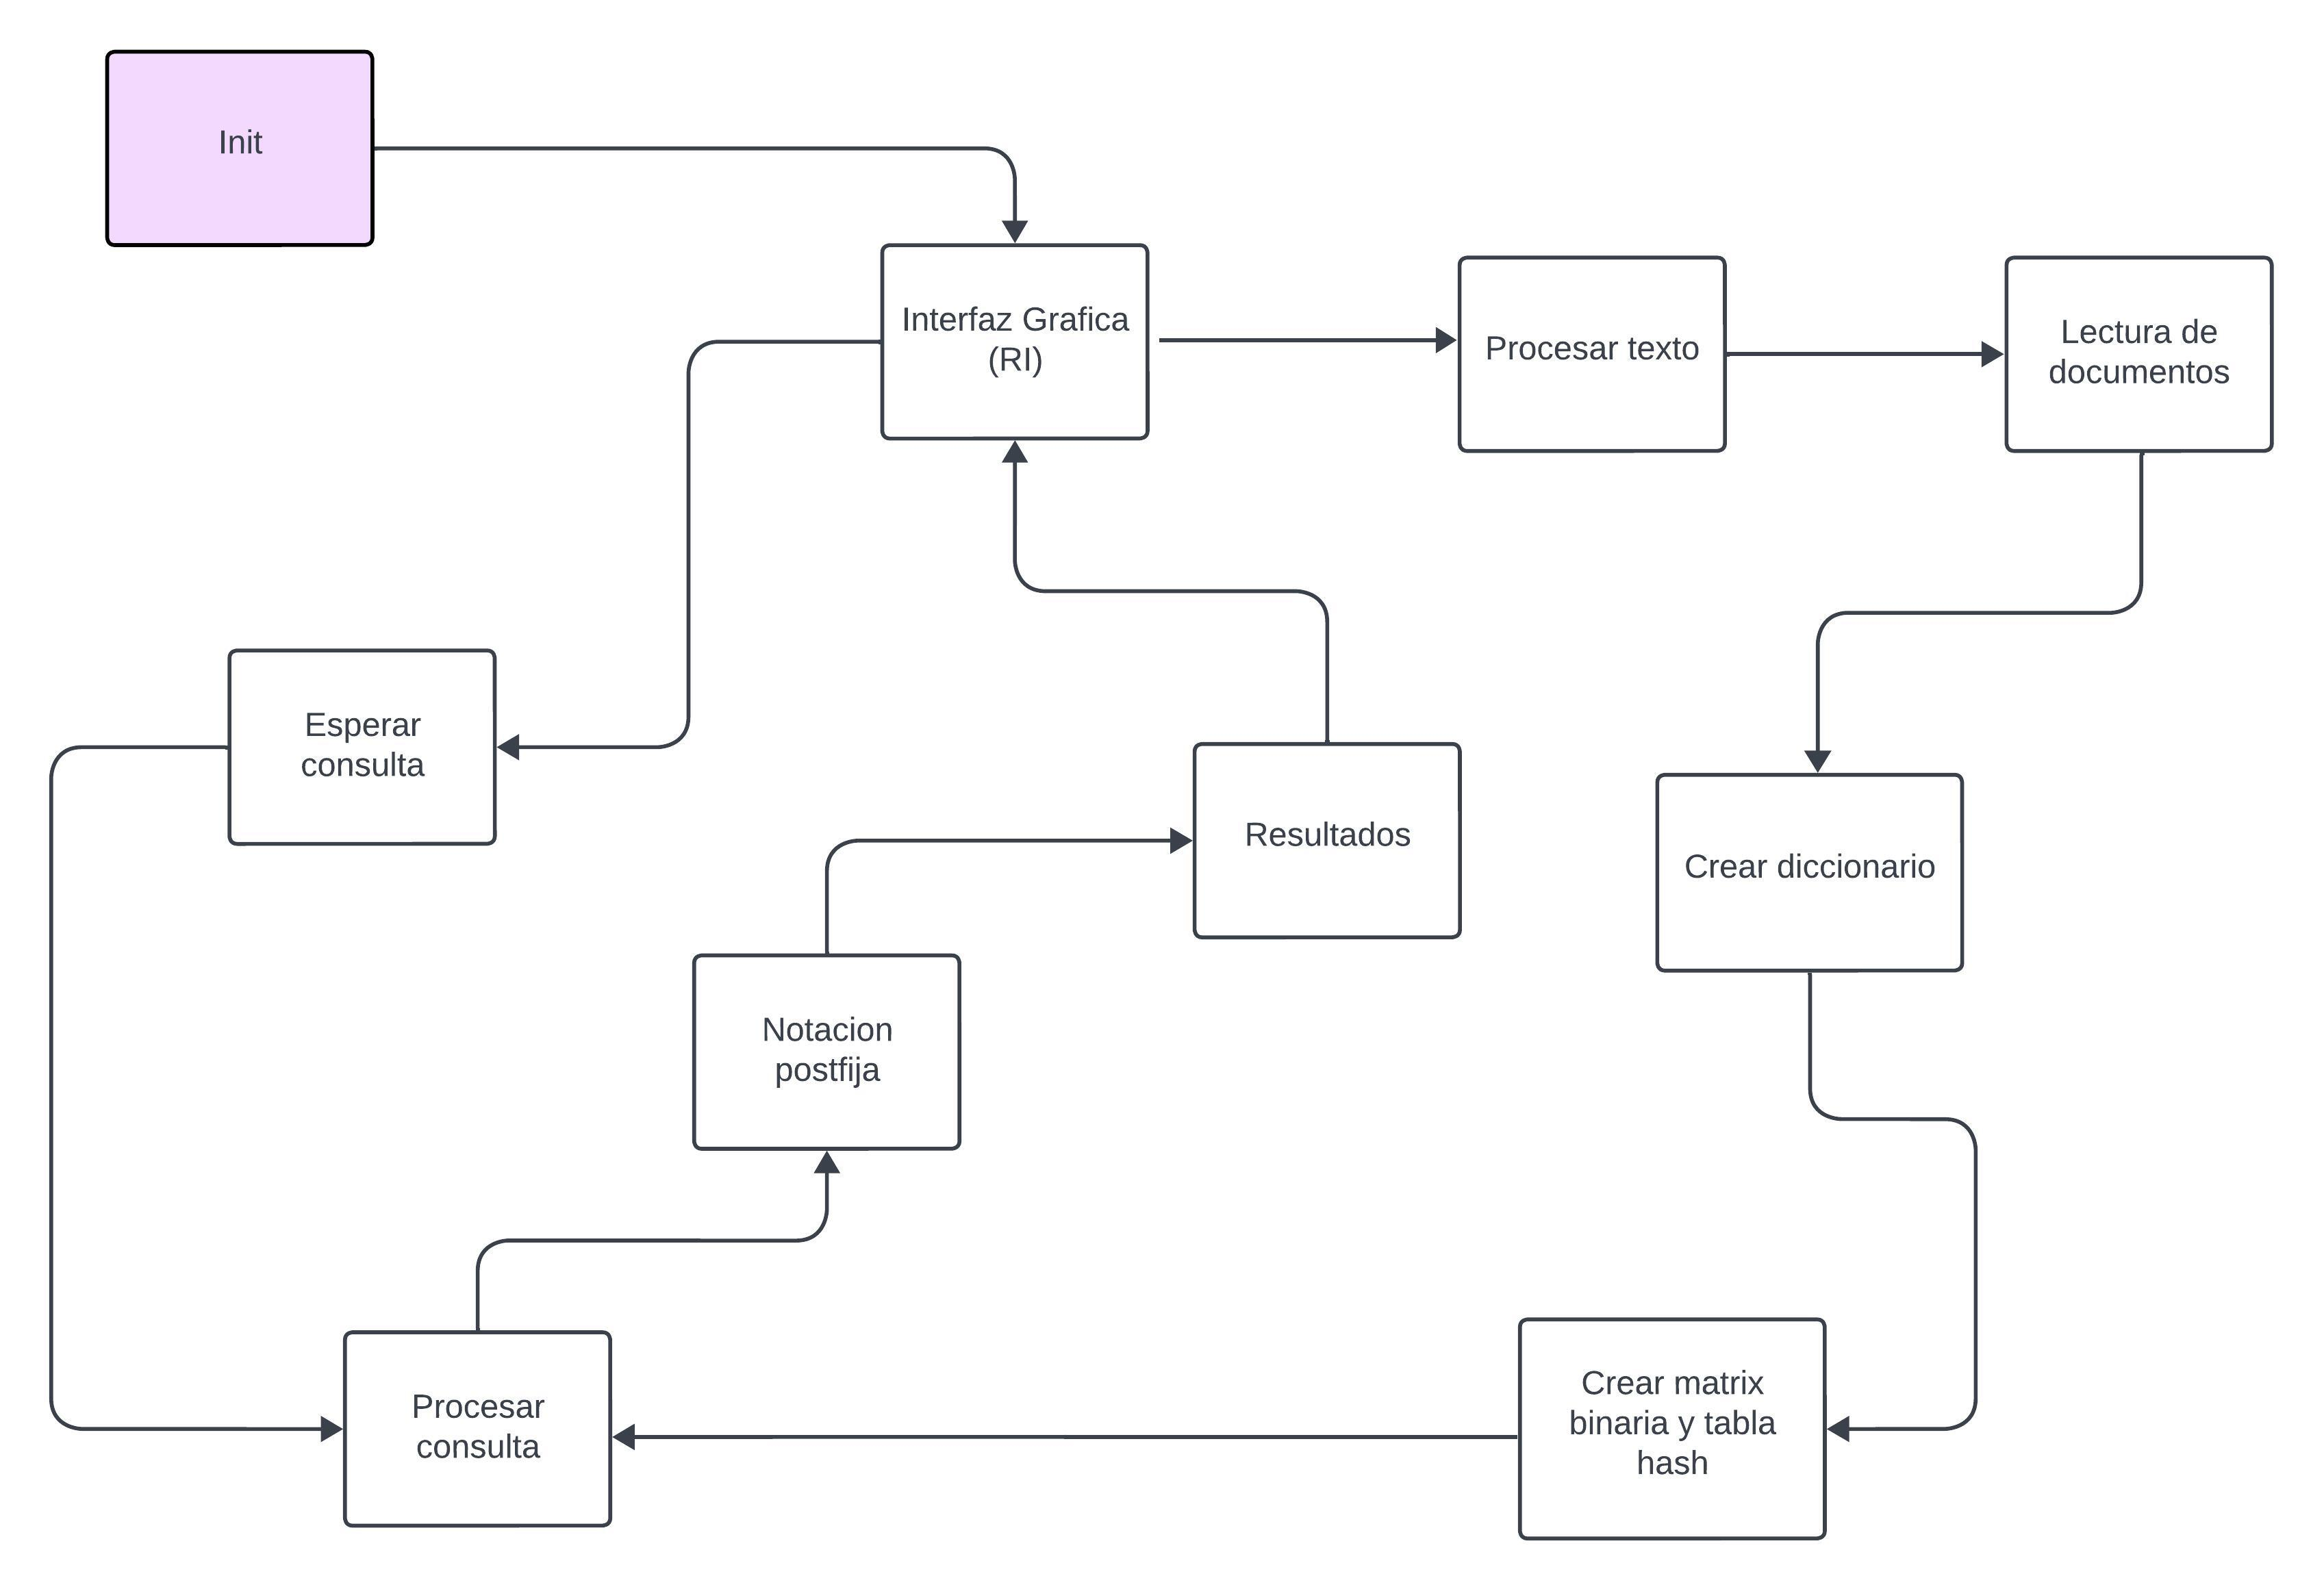
\includegraphics[width=0.8\textwidth]{src/img/ejecucion/7.jpg}
  \caption{Diagrama del sistema booleano}
\end{figure}
\subsection{Descripción de cada uno de los módulos del programa}

\begin{itemize}
  \item Init 
  \begin{itemize}
    \item init (self) \\ El constructor de la clase Sistema RI inicializa varios atributos y configuraciones necesarios para el sistema de recuperación de información (RI). Esto incluye la inicialización de la interfaz gráfica en un hilo separado.
    \item init gui thread(self) \\ Este método inicializa la interfaz gráfica en un hilo separado utilizando PyQt5. También conecta la señal de consulta de la interfaz a una ranura (slot) que maneja la recepción de consultas.
  \end{itemize}
  \item Interfaz Gráfica (RI) 
  \begin{itemize}
    \item init (self, sistema ri) \\ El constructor de la clase InterfazRI inicializa la interfaz gráfica de usuario (GUI) y recibe una instancia de SistemaRI como argumento para establecer una comunicación entre la interfaz y el sistema de recuperación de información.
    \item initUI(self) \\ Este método configura la interfaz de usuario utilizando la biblioteca PyQt5. Define la estructura de la ventana principal
    \item openDocument(self) \\ Abre un cuadro de diálogo para seleccionar y abrir un documento de texto. Luego, muestra el contenido del documento en el área de visualización.
    \item update document displayed(self, item) \\ Este método se llama cuando se hace clic en un elemento de la lista de resultados. Si el elemento hace referencia a un documento, muestra el contenido del documento seleccionado en el área de visualización.
    \item mostrar ayuda(self) \\ Muestra un cuadro de diálogo modal (QDialog) con información de ayuda sobre cómo usar la aplicación.
    \item closeEvent(self, event) \\ Este método maneja el evento de cierre de la ventana principal y asegura que la aplicación se cierre correctamente cuando se cierra la ventana.
  \end{itemize}
  \item Procesar texto
  \begin{itemize}
    \item procesar texto(self, contenido) \\ Este método recibe un contenido de texto, realiza una serie de transformaciones como convertir a minúsculas, eliminar caracteres especiales, quitar acentos y números, y tokenizar el texto en palabras. Luego, devuelve una lista de palabras procesadas.
    \item token stopw(self, string) \\ Realiza la tokenización, elimina las stopwords y aplica stemming a una cadena de texto.
  \end{itemize}
  \item Crear Diccionario
  \begin{itemize}
    \item crear tabla(self, array, nombre) \\ Este método crea una tabla a partir de un array y la almacena en un archivo de texto. Es utilizado para almacenar tablas de palabras, frecuencias, stopwords y stemming.
  \end{itemize}
  \item Crear Matriz Binaria y Tabla Hash
  \begin{itemize}
    \item crear matriz binaria(self, palabras, numero documentos) \\ Este método crea una matriz binaria donde cada fila representa una palabra y cada columna representa un documento. El valor en cada celda de la matriz indica si la palabra aparece en el documento correspondiente.
    \item computar hash(self, word) \\ Calcula el valor hash MD5 de una palabra y lo devuelve como una cadena hexadecimal.
    \item crear hash table(self, words, binary dict) \\ Crea una tabla hash que asocia palabras a sus valores binarios en la matriz binaria.
  \end{itemize}
  \item procesar consulta
  \begin{itemize}
    \item process query(self, operator) \\ Este método procesa una consulta booleana en notación infija y la convierte en notación postfija. Luego, ejecuta la consulta y muestra los resultados en la interfaz gráfica.
    \item hash query(self, hash) \\ Busca en la tabla hash un valor binario correspondiente a un hash de palabra.
    \item ejecutar query(self, postfijo) \\ Ejecuta una consulta booleana en notación postfija utilizando los arrays binarios y devuelve el resultado.
    \item obtener docs(self, array docs) \\ Imprime los documentos que satisfacen una consulta booleana en función del resultado de la evaluación.
    \item clear(self) \\ Limpia las variables y reinicia el sistema para una nueva consulta.
  \end{itemize}
  \item Notacion posfija
  \begin{itemize}
    \item procesar bool exp(self, query str) \\ Toma una cadena de consulta booleana y la convierte en una lista de elementos que representan la expresión booleana.
    \item procesar postfijo(self, bool exp list) \\ Toma una lista de elementos que representan la expresión booleana en notación infija y la convierte en notación postfija.
    \item or operator(self) \\ Implementa la operación lógica OR en listas binarias y devuelve el resultado.
    \item and operator(self) \\ Implementa la operación lógica AND en listas binarias y devuelve el resultado.
    \item not operator(self) \\ Implementa la operación lógica NOT en una lista binaria y devuelve el resultado.
  \end{itemize}
  \item Esperar consulta
  \begin{itemize}
    \item esperar consulta(self) \\ Bloquea hasta que se recibe una consulta desde la interfaz gráfica.
    \item recibir consulta(self, consulta) \\ Recibe una consulta desde la interfaz gráfica y la almacena para su posterior procesamiento.
  \end{itemize}
  \item Resultados
  \begin{itemize}
    \item enviar consulta(self) \\ Este método se llama cuando se hace clic en el botón ”Enviar”o se presiona la tecla Enter después de ingresar una consulta en el cuadro de texto. Toma la consulta ingresada por el usuario y la emite como una señal consulta signal para que el sistema de recuperación de información la procese.
    \item update output(self, output) \\ Este método agrega resultados a la lista de resultados en la interfaz gráfica.
  \end{itemize}
\end{itemize}